% (The MIT License)
%
% Copyright (c) 2023-2024 Yegor Bugayenko
%
% Permission is hereby granted, free of charge, to any person obtaining a copy
% of this software and associated documentation files (the 'Software'), to deal
% in the Software without restriction, including without limitation the rights
% to use, copy, modify, merge, publish, distribute, sublicense, and/or sell
% copies of the Software, and to permit persons to whom the Software is
% furnished to do so, subject to the following conditions:
%
% The above copyright notice and this permission notice shall be included in all
% copies or substantial portions of the Software.
%
% THE SOFTWARE IS PROVIDED 'AS IS', WITHOUT WARRANTY OF ANY KIND, EXPRESS OR
% IMPLIED, INCLUDING BUT NOT LIMITED TO THE WARRANTIES OF MERCHANTABILITY,
% FITNESS FOR A PARTICULAR PURPOSE AND NONINFRINGEMENT. IN NO EVENT SHALL THE
% AUTHORS OR COPYRIGHT HOLDERS BE LIABLE FOR ANY CLAIM, DAMAGES OR OTHER
% LIABILITY, WHETHER IN AN ACTION OF CONTRACT, TORT OR OTHERWISE, ARISING FROM,
% OUT OF OR IN CONNECTION WITH THE SOFTWARE OR THE USE OR OTHER DEALINGS IN THE
% SOFTWARE.

\documentclass{article}
\usepackage{../osbp}
\newcommand*\thetitle{Releasing}
\begin{document}

\plush{\osbpTitlePage{7}{}}

\qte
  [\nospell{Andre Van Der Hoek}]
  {andre-van-der-hoek}
  {Simply \ul{making available} and retrieving interdependent components individually \ul{neither} facilitates independent software development \ul{nor} encourages widespread use of large systems of systems.}
  {van1997software}

\qte
  [\nospell{G{\"u}nther Ruhe}]
  {gunther-ruhe}
  {Release planning is typically done \textit{ad hoc} and \ul{not} based on sound \ul{models and methodologies}. This is even the case when planning involves several hundred features.}
  {ruhe2005art}

\thought{Release when it's different, not when it's good.}

\qte
  [\nospell{Kazu Okumoto}]
  {kazu-okumoto}
  {\textbf{\nospell{Goel-Okumoto} model}: An important problem of practical concern is the determination of the point when testing should \ul{stop} and the system can be considered ready for release, that is, the determination of the \ul{software release time}. Two criteria are investigated: software reliability and total expected cost.}
  {okumoto1979optimum}

\qte
  [\nospell{Shigeru Yamada}]
  {shigeru-yamada}
  {This paper extends the problem of \citet{okumoto1979optimum} by evaluating \ul{both criteria} simultaneously. We discuss optimal software release policies which minimize a total average software cost under the constraint of satisfying a software reliability requirement.}
  {yamada1985cost}
\pitch{
  \begin{multicols}{2}
  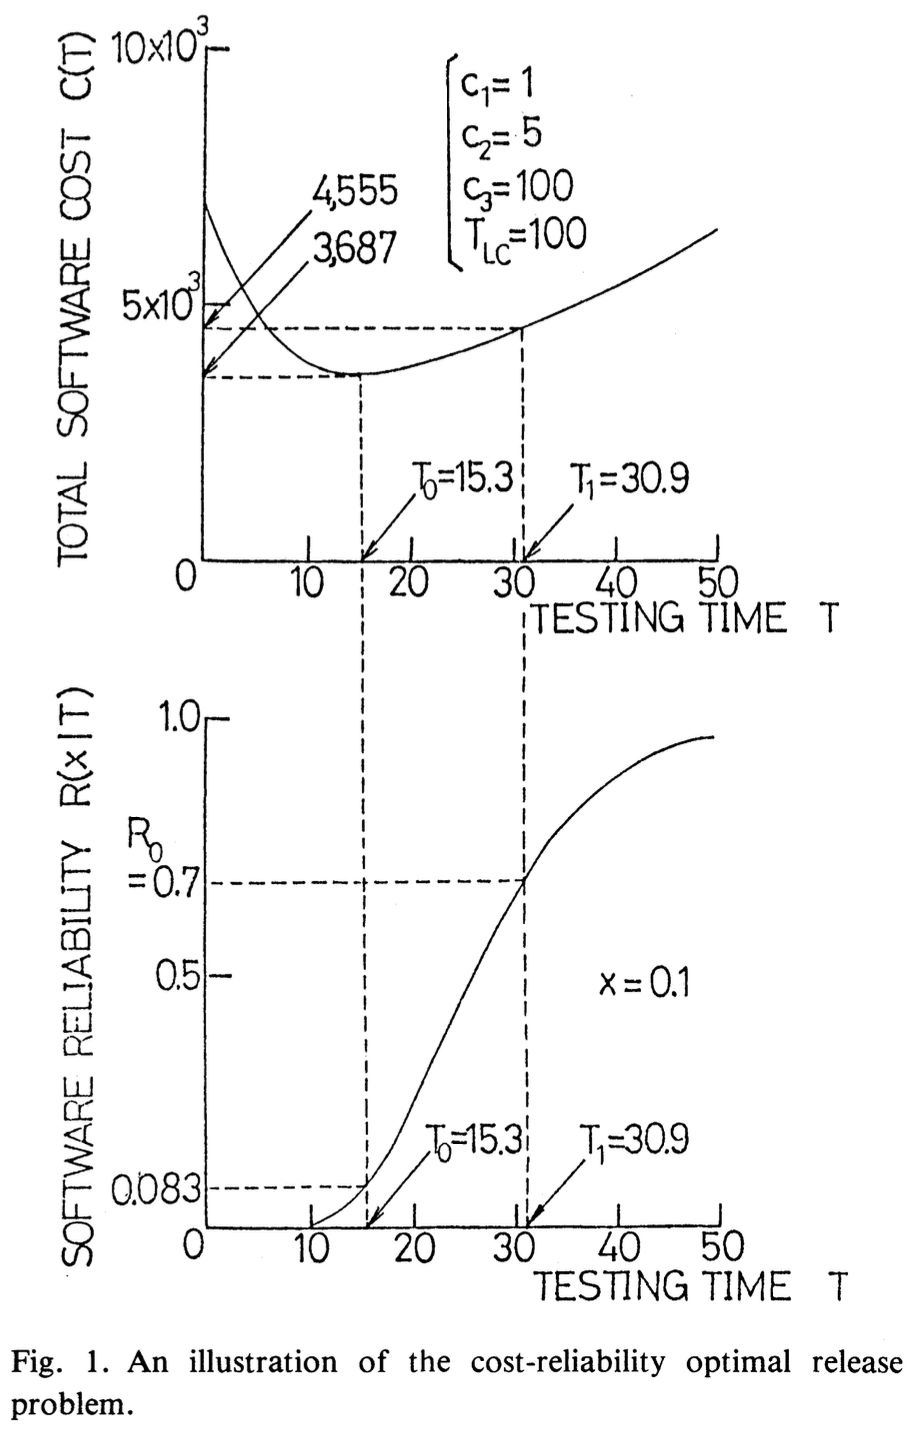
\includegraphics[width=.65\linewidth]{time-vs-cost.png}
  \par\columnbreak\par
  ``The optimum software release time is the testing time which comes closest to satisfying some pre-specified software reliability.''
  \source{yamada1985cost}
  \end{multicols}}

\thought{Fully automate the release process, avoiding any manual intervention.}

\qte
  [\nospell{Jez Humble}]
  {jez-humble}
  {Over time, deployments should tend towards being fully automated. There should be \ul{two tasks} for a human being to perform to deploy software into a development, test, or production environment: to pick the version and environment and to press the `deploy' button.}
  {humble2010continuous}

\thought{Release frequently.}

\qte
  [\nospell{Victor Basili}]
  {victor-basili}
  {If improving productivity is the main concern, then it may be wise to try to \ul{avoid} scheduling \ul{small} error correction releases. Instead the manager should try, when possible, to \ul{package} small error corrections in a release with larger enhancements.}
  {basili1996understanding}

\qte
  [\nospell{Foutse Khomh}]
  {foutse-khomh}
  {We found that (1)~with shorter release cycles, users do not experience significantly more post-release bugs and (2)~bugs are fixed faster, yet (3)~users experience these bugs earlier during software execution (the program crashes earlier).}
  {khomh2012faster}

\thought{Generate release notes automatically.}

\thought{Publish packages}


\thought{Be aware of malware.}

\thought{Announce them.}

\end{document}
